%\documentclass{beamer}
\documentclass[handout]{beamer}
\usetheme{Marburg}
\useoutertheme{infolines}
\newcommand{\answers}{1}

\usepackage{amsmath}
\usepackage{caption}
\usepackage{color}
\usepackage{enumerate}
\usepackage{listings}
\usepackage{hyperref}
\usepackage{mathrsfs}
\usepackage{natbib}
\usepackage{url}

\providecommand{\all}{\ \forall \ }
\providecommand{\bs}{\backslash}
\providecommand{\e}{\varepsilon}
\providecommand{\E}{\ \exists \ }
\providecommand{\lm}[2]{\lim_{#1 \rightarrow #2}}
\providecommand{\m}[1]{\mathbb{#1}}
\providecommand{\nv}{{}^{-1}}
\providecommand{\ov}[1]{\overline{#1}}
\providecommand{\p}{\newpage}
\providecommand{\q}{$\quad$ \newline}
\providecommand{\rt}{\rightarrow}
\providecommand{\Rt}{\Rightarrow}
\providecommand{\vc}[1]{\boldsymbol{#1}}
\providecommand{\wh}[1]{\widehat{#1}}

\hypersetup{colorlinks,linkcolor=,urlcolor=blue}
\numberwithin{equation}{section}

\definecolor{dkgreen}{rgb}{0,0.6,0}
\definecolor{gray}{rgb}{0.5,0.5,0.5}
\definecolor{mauve}{rgb}{0.58,0,0.82}

\lstset{ 
  language=C,                % the language of the code
  basicstyle= \footnotesize,           % the size of the fonts that are used for the code
  numbers=left,
  numberfirstline=true,
  numbersep=5pt,                  % how far the line-numbers are from the code
  backgroundcolor=\color{white},      % choose the background color. You must add \usepackage{color}
  showspaces=false,               % show spaces adding particular underscores
  showstringspaces=false,         % underline spaces within strings
  showtabs=false,                 % show tabs within strings adding particular underscores
  frame=lrb,                   % adds a frame around the code
  rulecolor=\color{black},        % if not set, the frame-color may be changed on line-breaks within not-black text 
  tabsize=2,                      % sets default tabsize to 2 spaces
  captionpos=t,                   % sets the caption-position 
  breaklines=true,                % sets automatic line breaking
  breakatwhitespace=false,        % sets if automatic breaks should only happen at whitespace
  %title=\lstname,                   % show the filename of files included with \lstinputlisting;
  keywordstyle=\color{blue},          % keyword style
  commentstyle=\color{gray},       % comment style
  stringstyle=\color{dkgreen},         % string literal style
  escapeinside={\%*}{*)},            % if you want to add LaTeX within your code
  morekeywords={*, ...},               % if you want to add more keywords to the set
  xleftmargin=0.2in, % left horizontal offset of caption box
  xrightmargin=-.03in % right horizontal offset of caption box
}

%\DeclareCaptionFont{white}{\color{white}}
%\DeclareCaptionFormat{listing}{\parbox{\textwidth}{\colorbox{gray}{\parbox{\textwidth}{#1#2#3}}\vskip-0.05in}}
%\captionsetup[lstlisting]{format = listing, labelfont = white, textfont = white}
%For caption-free listings, comment out the 3 lines above and uncomment the 2 lines below.
 \captionsetup{labelformat = empty, labelsep = none}
 \lstset{frame = single}

\title{CUDA C: race conditions, atomics, locks, mutex, and warps}
\author{Will Landau}
\date{October 21, 2013}
\institute{Iowa State University}

\begin{document}

\begin{frame}
\titlepage
 \end{frame}
 
 \begin{frame}
\frametitle{Outline}
\tableofcontents
\end{frame}
 
 \AtBeginSection[]
{
   \begin{frame}
       \frametitle{Outline}
       \tableofcontents[currentsection]
   \end{frame}
}

\section{Race conditions}

\begin{frame}
\frametitle{Race conditions}
\begin{itemize}
\item Let {\tt int *x} point to global memory. {\tt *x++} happens in 3 steps:
\begin{enumerate}
\pause \item Read the value in {\tt *x} into a register.
\pause \item Add 1 to the value read in step 1.
\pause \item Write the result back to {\tt *x}.
\end{enumerate}
\pause \item If we want parallel threads A and B to both increment {\tt *x}, then we want something like:
\begin{enumerate}
\pause \item Thread A reads the value, 7, from {\tt *x}.
\pause \item Thread A adds 1 to its value, 7, to make 8.
\pause \item Thread A writes its value, 8, back to {\tt *x}.
\pause \item Thread B reads the value, 8, from {\tt *x}.
\pause \item Thread B adds 1 to its value, 8, to make 9.
\pause \item Thread B writes the value, 9, back to {\tt *x}.
\end{enumerate}
\end{itemize}
\end{frame}

\begin{frame}
\frametitle{Race conditions}
\begin{itemize}
\item But since the threads are parallel, we might actually get:
\begin{enumerate}
\pause \item Thread A reads the value, 7, from {\tt *x}.
\pause \item Thread B reads the value, 7, from {\tt *x}.
\pause \item Thread A adds 1 to its value, 7, to make 8.
\pause \item Thread A writes its value, 8, back to {\tt *x}.
\pause \item Thread B adds 1 to its value, 7, to make 8.
\pause \item Thread B writes the value, 8, back to {\tt *x}.
\end{enumerate}
\end{itemize}
\end{frame}


\begin{frame}[fragile]
\frametitle{Example: {\tt race\_condition.cu}} \lstset{basicstyle=\tiny}
\begin{lstlisting}[name=racecon]
#include <stdio.h>
#include <stdlib.h>
#include <cuda.h>
#include <cuda_runtime.h> 

__global__ void colonel(int *a_d){
  *a_d += 1;
}

int main(){

  int a = 0, *a_d;
  
  cudaMalloc((void**) &a_d, sizeof(int));
  cudaMemcpy(a_d, &a, sizeof(int), cudaMemcpyHostToDevice);

  float   elapsedTime;
  cudaEvent_t start, stop;
  cudaEventCreate(&start);
  cudaEventCreate(&stop);
  cudaEventRecord( start, 0 );
  
  colonel<<<1000,1000>>>(a_d); 
\end{lstlisting}
\end{frame}

\begin{frame}[fragile]
\frametitle{Example: {\tt race\_condition.cu}} \lstset{basicstyle=\tiny}
\begin{lstlisting}[name=racecon]
  cudaEventRecord( stop, 0 );
  cudaEventSynchronize( stop );
  cudaEventElapsedTime( &elapsedTime, start, stop );
  cudaEventDestroy( start );
  cudaEventDestroy( stop );
  printf("GPU Time elapsed: %f seconds\n", elapsedTime/1000.0);
  
  
  cudaMemcpy(&a, a_d, sizeof(int), cudaMemcpyDeviceToHost);

  printf("a = %d\n", a);
  cudaFree(a_d);

}
\end{lstlisting}

\begin{lstlisting}
> nvcc race_condition.cu -o race_condition
> ./race_condition
GPU Time elapsed: 0.000148 seconds
a = 88
\end{lstlisting}
\begin{itemize}
\pause \item Since we started with {\tt a} at 0, we should have gotten {\tt a $= 1000 \cdot 1000 = 1,000,000$}.
\end{itemize}
\end{frame}


\begin{frame}
\frametitle{Race conditions}
\begin{itemize}
\pause \item {\bf Race condition}: A computational hazard that arises when the results of the program depend on the timing of uncontrollable events, such as the execution order or threads.
\begin{itemize}
\pause \item Many race conditions are caused by violations of the SIMD paradigm.
\pause \item Atomic operations and locks are brute force ways to fix race conditions.
\end{itemize}
\end{itemize}
\end{frame}

\section{Brute force fixes: atomics, locks, and mutex}

\begin{frame}[fragile]
\frametitle{Atomics}
\begin{itemize}
\item {\bf Atomic operation}: an operation that forces otherwise parallel threads into a bottleneck, executing the operation one at a time. 
\pause \item In {\tt colonel()}, replace
\begin{align*}
\text{\tt *a\_d += 1;}
\end{align*}
\pause with an atomic function,
\begin{align*}
\text{\tt atomicAdd(a\_d, 1);}
\end{align*}
to fix the race condition in {\tt race\_condition.cu}.
\end{itemize}
\end{frame}

\begin{frame}[fragile]
\frametitle{{\tt race\_condition\_fixed.cu}} \lstset{basicstyle=\tiny}
\begin{lstlisting}[name=rfix]
#include <stdio.h>
#include <stdlib.h>
#include <cuda.h>
#include <cuda_runtime.h> 

__global__ void colonel(int *a_d){
  atomicAdd(a_d, 1);
}

int main(){

  int a = 0, *a_d;
  
  cudaMalloc((void**) &a_d, sizeof(int));
  cudaMemcpy(a_d, &a, sizeof(int), cudaMemcpyHostToDevice);

  float   elapsedTime;
  cudaEvent_t start, stop;
  cudaEventCreate(&start);
  cudaEventCreate(&stop);
  cudaEventRecord( start, 0 );

  colonel<<<1000,1000>>>(a_d); 
\end{lstlisting}
\end{frame}

\begin{frame}[fragile]
\frametitle{{\tt race\_condition\_fixed.cu}} \lstset{basicstyle=\tiny}
\begin{lstlisting}[name=rfix]
  cudaEventRecord( stop, 0 );
  cudaEventSynchronize( stop );
  cudaEventElapsedTime( &elapsedTime, start, stop );
  cudaEventDestroy( start );
  cudaEventDestroy( stop );
  printf("GPU Time elapsed: %f seconds\n", elapsedTime/1000.0);
  
  
  cudaMemcpy(&a, a_d, sizeof(int), cudaMemcpyDeviceToHost);

  printf("a = %d\n", a);
  cudaFree(a_d);

}
\end{lstlisting}
\end{frame}

\begin{frame}[fragile]
\frametitle{{\tt race\_condition\_fixed.cu}} 
\begin{lstlisting}
> nvcc race_condition_fixed.cu -arch sm_20 -o race_condition_fixed
> ./race_doncition_fixed
GPU Time elapsed: 0.01485 seconds
a = 1000000
\end{lstlisting}
\begin{itemize}
\pause \item We got the right answer this time, and execution was slower because we forced the threads to execute the addition sequentially.
\pause \item If you're using builtin atomic functions like {\tt atomicAdd()}, use the {\tt -arch sm\_20} flag in compilation. 
\begin{itemize}
\pause \item This is to make sure you're using CUDA compute capability (version) 2.0 or above.
\end{itemize}
\end{itemize}
\end{frame}

\begin{frame}
\frametitle{CUDA C builtin atomic functions}

\begin{itemize}
\item With CUDA compute capability 2.0 or above, you can use:
\begin{itemize}
\item {\tt atomicAdd()}
\item {\tt atomicSub()}
\item {\tt atomicMin()}
\item {\tt atomicMax()}
\item {\tt atomicInc()}
\item {\tt atomicDec()}
\item {\tt atomicAdd()}
\item {\tt atomicExch()}
\item {\tt atomicCAS()}
\item {\tt atomicAnd()}
\item {\tt atomicOr()}
\item {\tt atomicXor()}
\end{itemize}
\pause \item For documentation, refer to the \href{http://docs.nvidia.com/cuda/cuda-c-programming-guide/index.html}{CUDA C programming guide}.
\end{itemize}
\end{frame}


\begin{frame}
\frametitle{{\tt atomicCAS(int *address, int compare, int val)}: needed for locks}
\begin{enumerate}
\pause \item Read the value, {\tt old}, located at {\tt address}.
\pause \item {\tt *address = (old == compare) ? val : old;}
\pause \item Return {\tt old}.
\end{enumerate}
\end{frame}

\begin{frame}[fragile]
\frametitle{Locks and mutex}
\begin{itemize}
\item {\bf Lock}: a mechanism in parallel computing that forces an entire segment of code to be executed atomically.
\pause \item {\bf mutex}
\begin{itemize}
\pause \item ``mutual exclusion", the principle behind locks.
\pause \item While a thread is running code inside a lock, it shuts all the other threads out of the lock.
\end{itemize}
\end{itemize}

\pause \begin{lstlisting}
__global__ void someKernel(void){
  Lock myLock; 
  
  // some parallel code
  
  mylock.lock();
  // some sequential code
  mylock.unlock();
  
  // some parallel code
}
\end{lstlisting}
\end{frame}

\begin{frame}
\frametitle{The concept}
\begin{center}
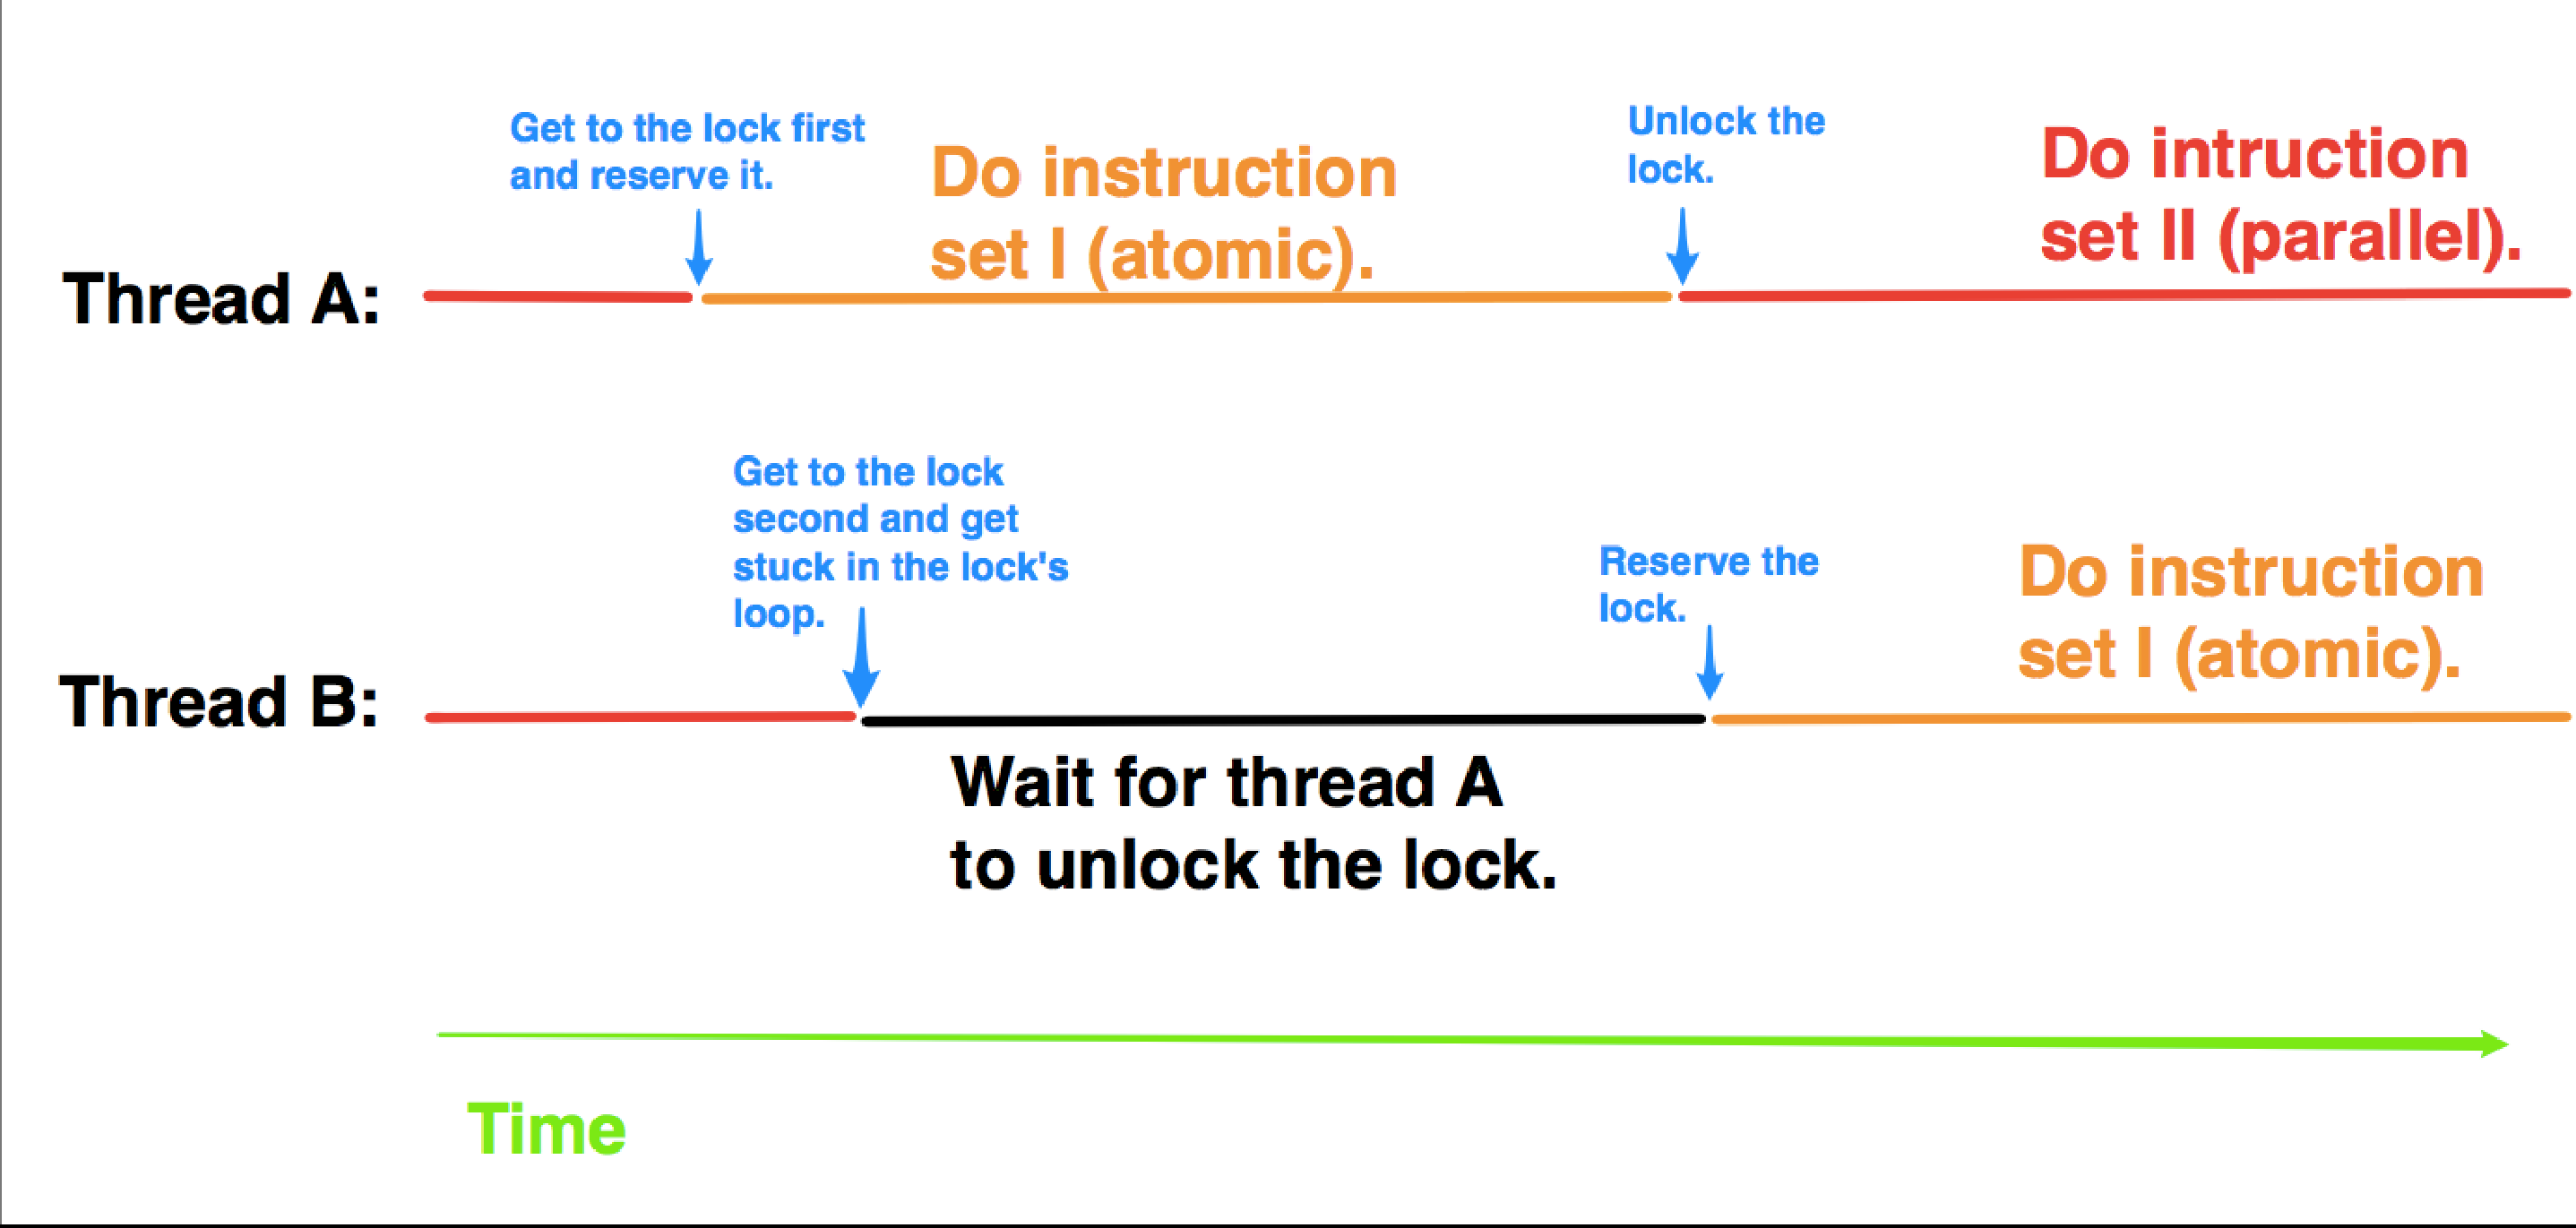
\includegraphics[scale=.2]{../../fig/lockconcept}
\end{center}
\end{frame}

\begin{frame}[fragile]
\frametitle{{\tt Lock.h}} \lstset{basicstyle=\tiny}
\begin{lstlisting}
struct Lock {
  int *mutex;
  
  Lock(){
    int state = 0;

    cudaMalloc((void**) &mutex, sizeof(int)));
    cudaMemcpy(mutex, &state, sizeof(int), cudaMemcpyHostToDevice));
  }
  
  ~Lock(){
    cudaFree(mutex);
  }

  __device__ void lock(){
    while(atomicCAS(mutex, 0, 1) != 0);
  }
  
  __device__ void unlock(){
    atomicExch(mutex, 0);
  }  
  
};
\end{lstlisting}
\end{frame}

\begin{frame}[fragile]
\frametitle{A closer look at the lock function}
\begin{lstlisting}[firstnumber=15]
__device__ void lock(){
  while(atomicCAS(mutex, 0, 1) != 0);
}
\end{lstlisting}

\begin{itemize}
\pause \item In pseudocode:
\end{itemize}

\lstset{basicstyle=\tiny}

\begin{lstlisting}
__device void lock(){
  repeat{
    do atomically{
      
      if(mutex == 0){
        mutex = 1;
        return_value = 0;
      }
      
      else if(mutex == 1){
        return_value = 1;
      }
    } // do atomically
    
    if(return_value == 0)
      exit loop;

  } // repeat
} // lock

\end{lstlisting}
\end{frame}



\begin{frame}[fragile]
\frametitle{Example: counting the number of blocks}

\begin{itemize}
\pause \item Compare the two kernels:
\end{itemize}



\pause \begin{lstlisting}[firstnumber=5]
__global__ void blockCounterUnlocked(int *nblocks){
  if(threadIdx.x == 0){
    *nblocks = *nblocks + 1;
  }
}
\end{lstlisting}

\pause \begin{lstlisting}[firstnumber=11]
__global__ void blockCounter1(Lock lock, int *nblocks){
  if(threadIdx.x == 0){
    lock.lock();
    *nblocks = *nblocks + 1;
    lock.unlock();
  }
}
\end{lstlisting}
\end{frame}





\begin{frame}[fragile]
\frametitle{\tt blockCounter.cu} \lstset{basicstyle=\tiny}
\begin{lstlisting}[name=bc]
#include "../common/lock.h"
#define NBLOCKS_TRUE 512
#define NTHREADS_TRUE 512 * 2

__global__ void blockCounterUnlocked( int *nblocks ){
   if(threadIdx.x == 0){
    *nblocks = *nblocks + 1;
  }
}

__global__ void blockCounter1( Lock lock, int *nblocks ){
  if(threadIdx.x == 0){
    lock.lock();
    *nblocks = *nblocks + 1;
    lock.unlock();
  }
}

int main(){
  int nblocks_host, *nblocks_dev;
  Lock lock;
  float elapsedTime;
  cudaEvent_t start, stop;
 
  cudaMalloc((void**) &nblocks_dev, sizeof(int));
  
  //blockCounterUnlocked:

  nblocks_host = 0;
  cudaMemcpy( nblocks_dev, &nblocks_host, sizeof(int), cudaMemcpyHostToDevice );
  
\end{lstlisting}
\end{frame}

\begin{frame}[fragile]
\frametitle{\tt blockCounter.cu} \lstset{basicstyle=\tiny}
\begin{lstlisting}[name=bc]
  cudaEventCreate(&start);
  cudaEventCreate(&stop);
  cudaEventRecord( start, 0 );

  blockCounterUnlocked<<<NBLOCKS_TRUE, NTHREADS_TRUE>>>(nblocks_dev);

  cudaEventRecord( stop, 0 );
  cudaEventSynchronize( stop );
  cudaEventElapsedTime( &elapsedTime, start, stop );

  cudaEventDestroy( start );
  cudaEventDestroy( stop ); 

  cudaMemcpy( &nblocks_host, nblocks_dev, sizeof(int), cudaMemcpyDeviceToHost );
  printf("blockCounterUnlocked <<< %d, %d >>> () counted %d blocks in %f ms.\n", 
        NBLOCKS_TRUE,
        NTHREADS_TRUE,
        nblocks_host,
        elapsedTime);
\end{lstlisting}
\end{frame}

\begin{frame}[fragile]
\frametitle{\tt blockCounter.cu} \lstset{basicstyle=\tiny}
\begin{lstlisting}[name=bc]
  //blockCounter1:

  nblocks_host = 0;
  cudaMemcpy( nblocks_dev, &nblocks_host, sizeof(int), cudaMemcpyHostToDevice );
  
  cudaEventCreate(&start);
  cudaEventCreate(&stop);
  cudaEventRecord( start, 0 );
  
  blockCounter1<<<NBLOCKS_TRUE, NTHREADS_TRUE>>>(lock, nblocks_dev);

  cudaEventRecord( stop, 0 );
  cudaEventSynchronize( stop );
  cudaEventElapsedTime( &elapsedTime, start, stop );

  cudaEventDestroy( start );
  cudaEventDestroy( stop ); 
  
  cudaMemcpy( &nblocks_host, nblocks_dev, sizeof(int), cudaMemcpyDeviceToHost );
  printf("blockCounter1 <<< %d, %d >>> () counted %d blocks in %f ms.\n", 
        NBLOCKS_TRUE,
        NTHREADS_TRUE,
        nblocks_host,
        elapsedTime);      
                   
  cudaFree(nblocks_dev); 
}
\end{lstlisting}
\end{frame}


\begin{frame}[fragile]
\frametitle{\tt blockCounter.cu}  \lstset{basicstyle=\tiny}
\begin{lstlisting}[name=bc]
> nvcc blockCounter.cu -arch sm_20 -o blockCounter
> ./blockCounter
blockCounterUnlocked <<< 512, 1024 >>> () counted 47 blocks in 0.057920 ms.
blockCounter1 <<< 512, 1024 >>> () counted 512 blocks in 0.636064 ms.
\end{lstlisting}
\end{frame}


\begin{frame}[fragile]
\frametitle{{\tt blockCounter.cu} pauses indefinitely with this kernel}
\begin{lstlisting}
__global__ void blockCounter2(Lock lock, int *nblocks){
  lock.lock();
  if(threadIdx.x == 0){
    *nblocks = *nblocks + 1;
  }
  lock.unlock();
}
\end{lstlisting}
\begin{itemize}
\pause \item Why? warps.
\end{itemize}
\end{frame}

\section{Warps}

\begin{frame}
\frametitle{Warps}
\begin{itemize}
\item {\tt Warp}: a group of 32 threads in the same block that execute in lockstep.
\begin{itemize}
\pause \item That is, they synchronize after every step (as if {\tt \_\_syncthreads()} is called as often as possible).
\pause \item All blocks are partitioned into warps.
\end{itemize}
\end{itemize}
\pause \begin{center}
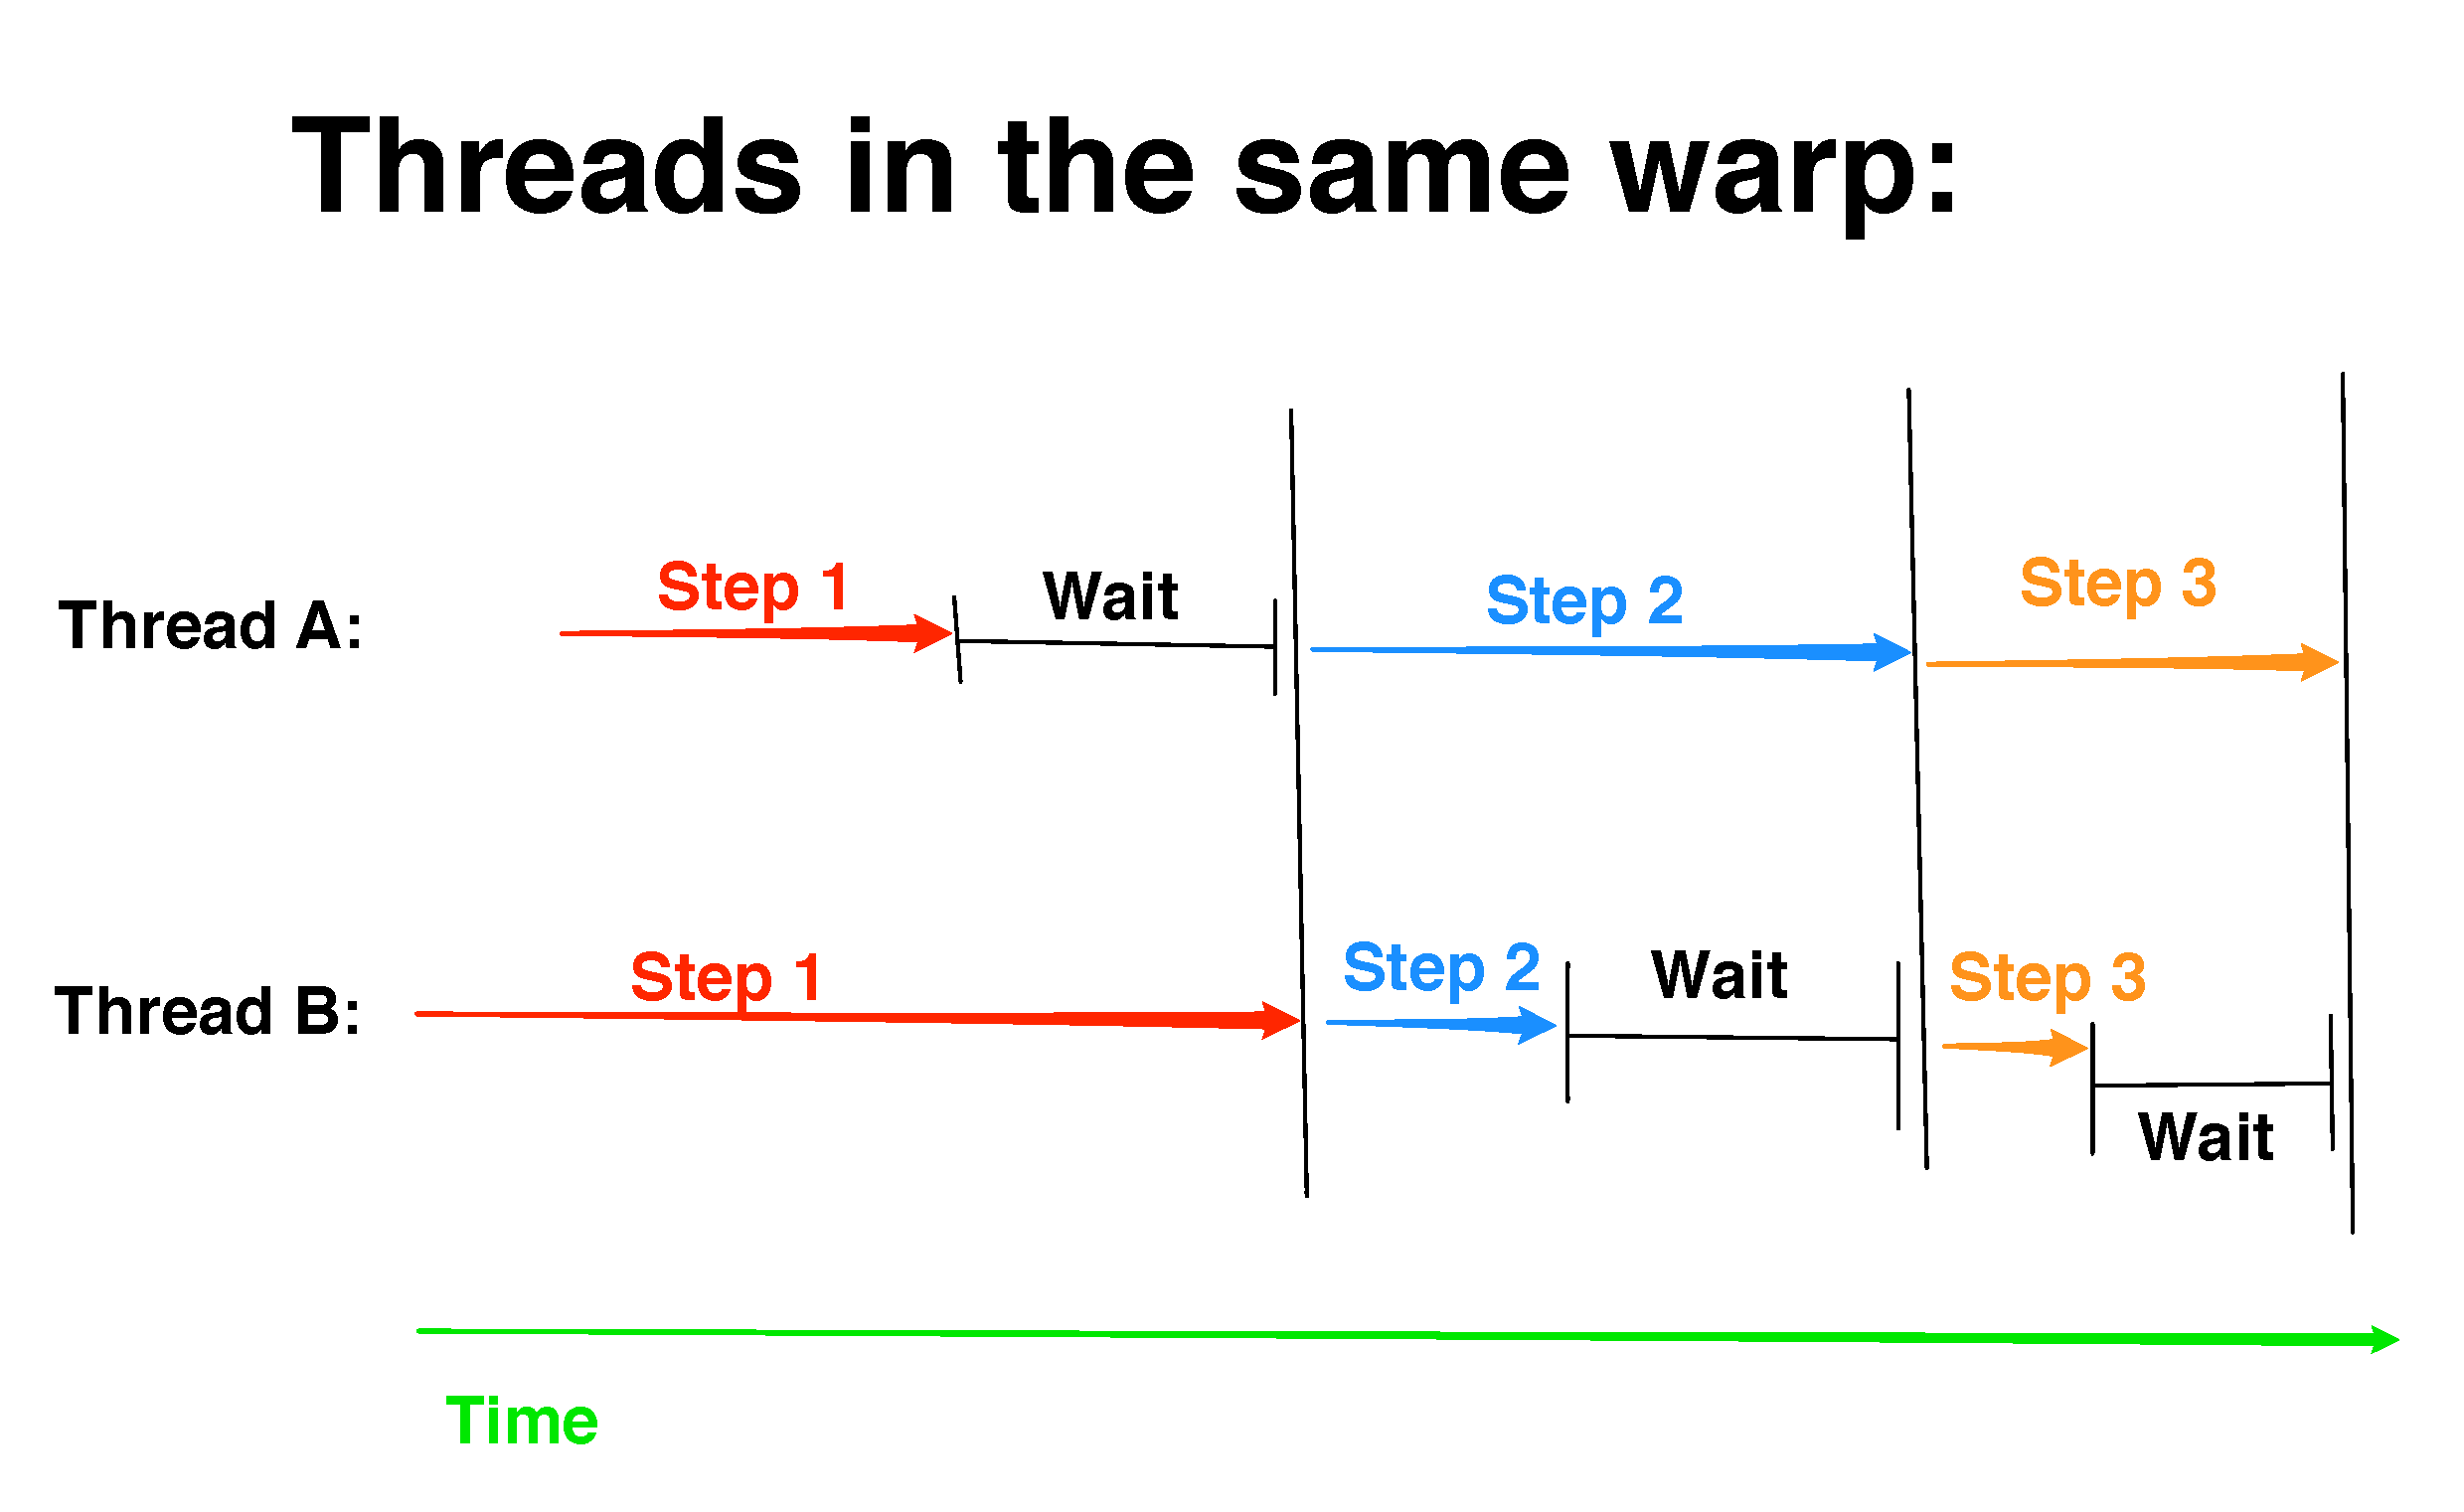
\includegraphics[scale=.2]{../../fig/samewarp}
\end{center}
\end{frame}

\begin{frame}
\frametitle{Warps}
 \begin{center}
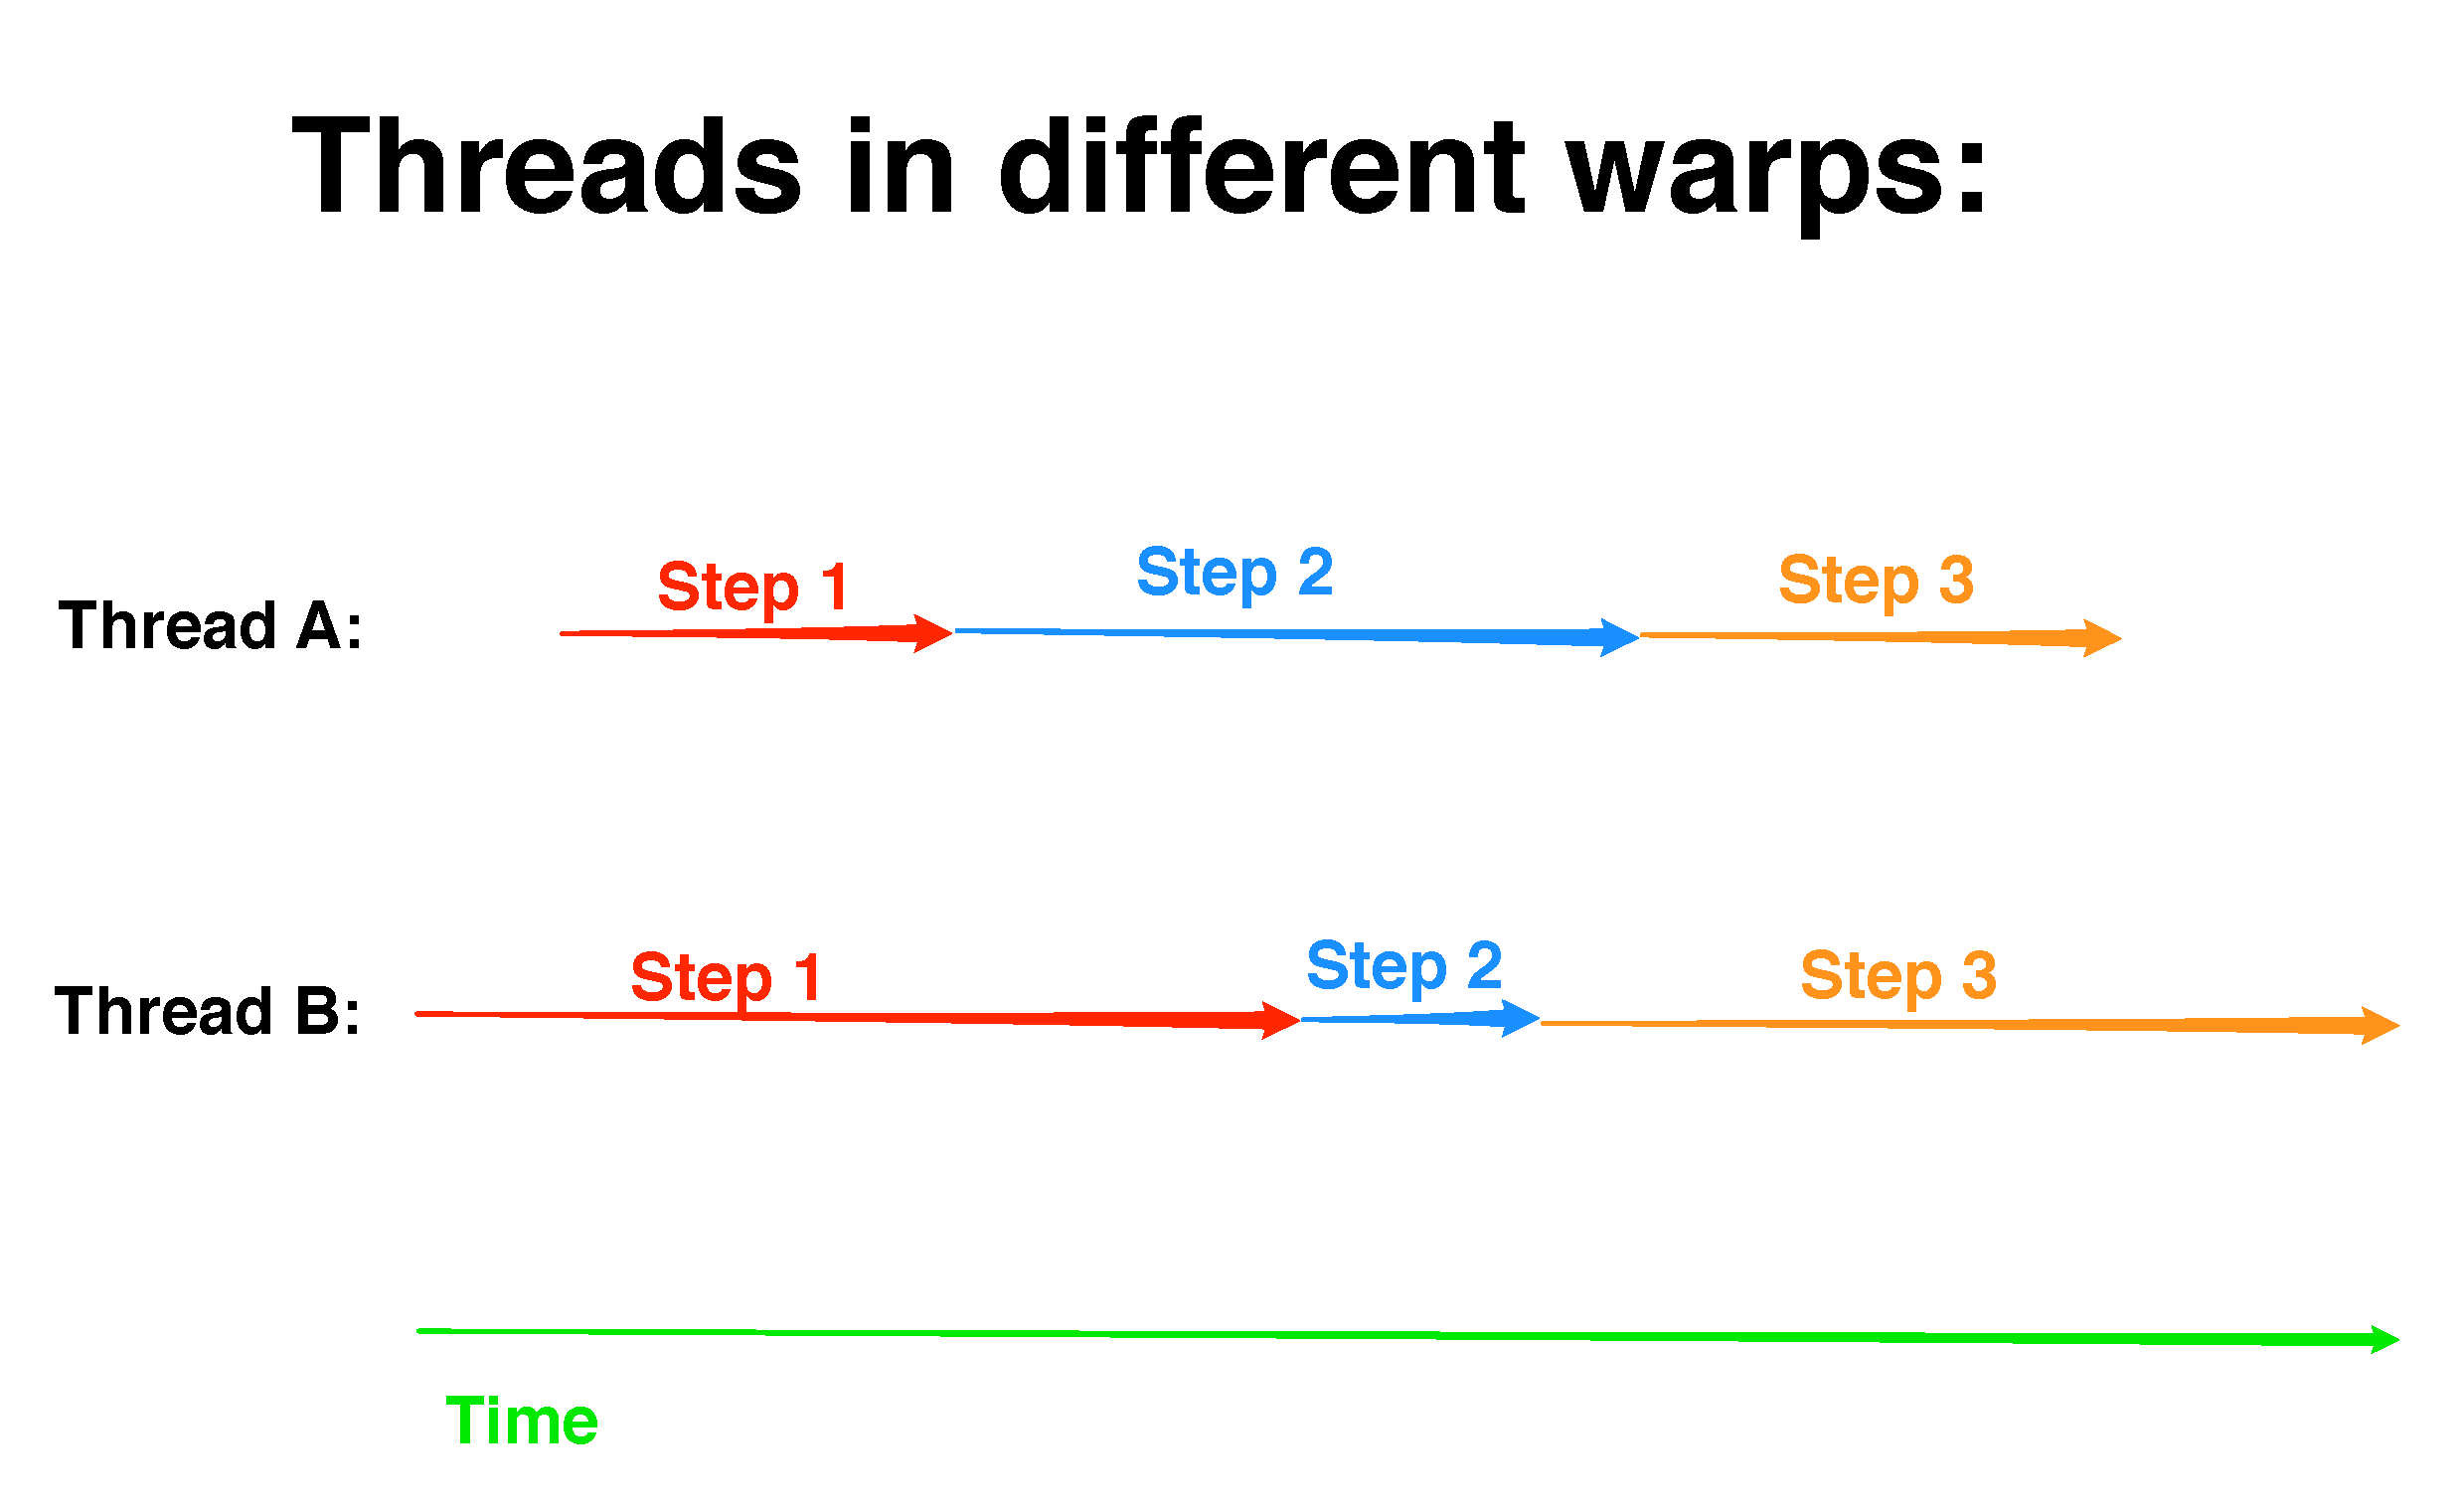
\includegraphics[scale=.2]{../../fig/diffwarp}
\end{center}
\end{frame}

\begin{frame}
\frametitle{Warps and locks}
 \begin{center}
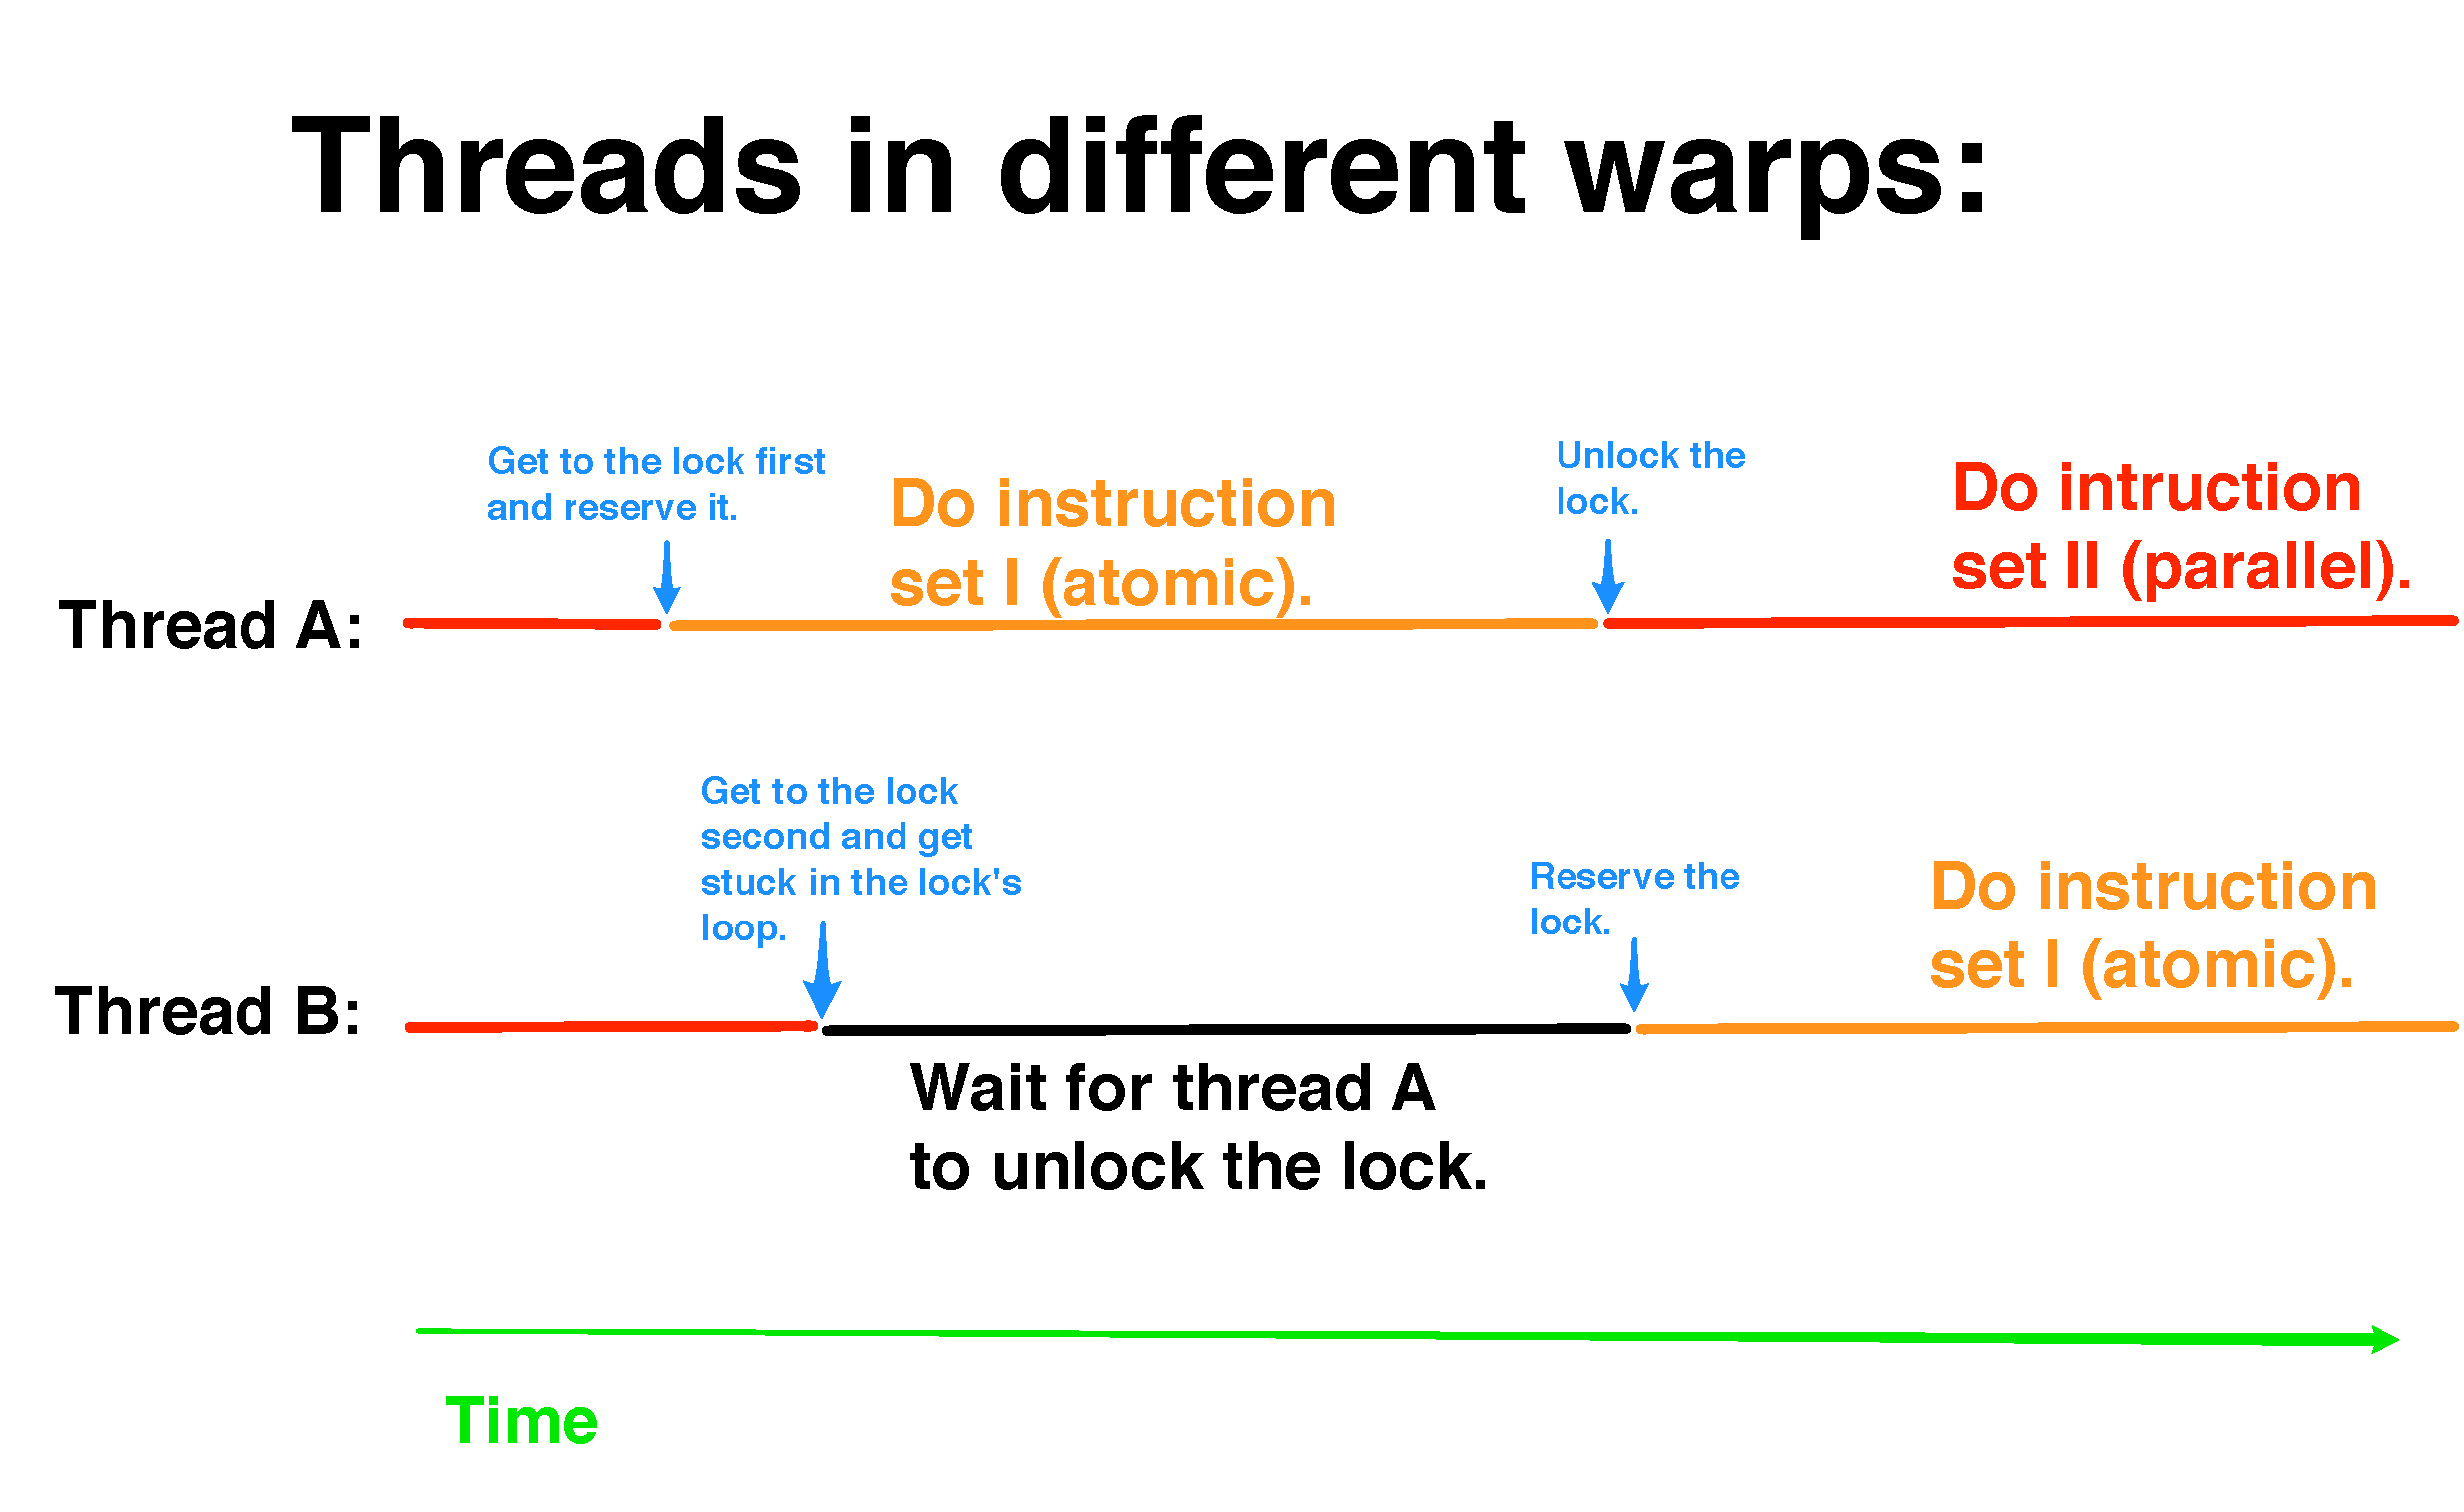
\includegraphics[scale=.2]{../../fig/lockwarp1}
\end{center}
\end{frame}

\begin{frame}
\frametitle{Warps and locks}
 \begin{center}
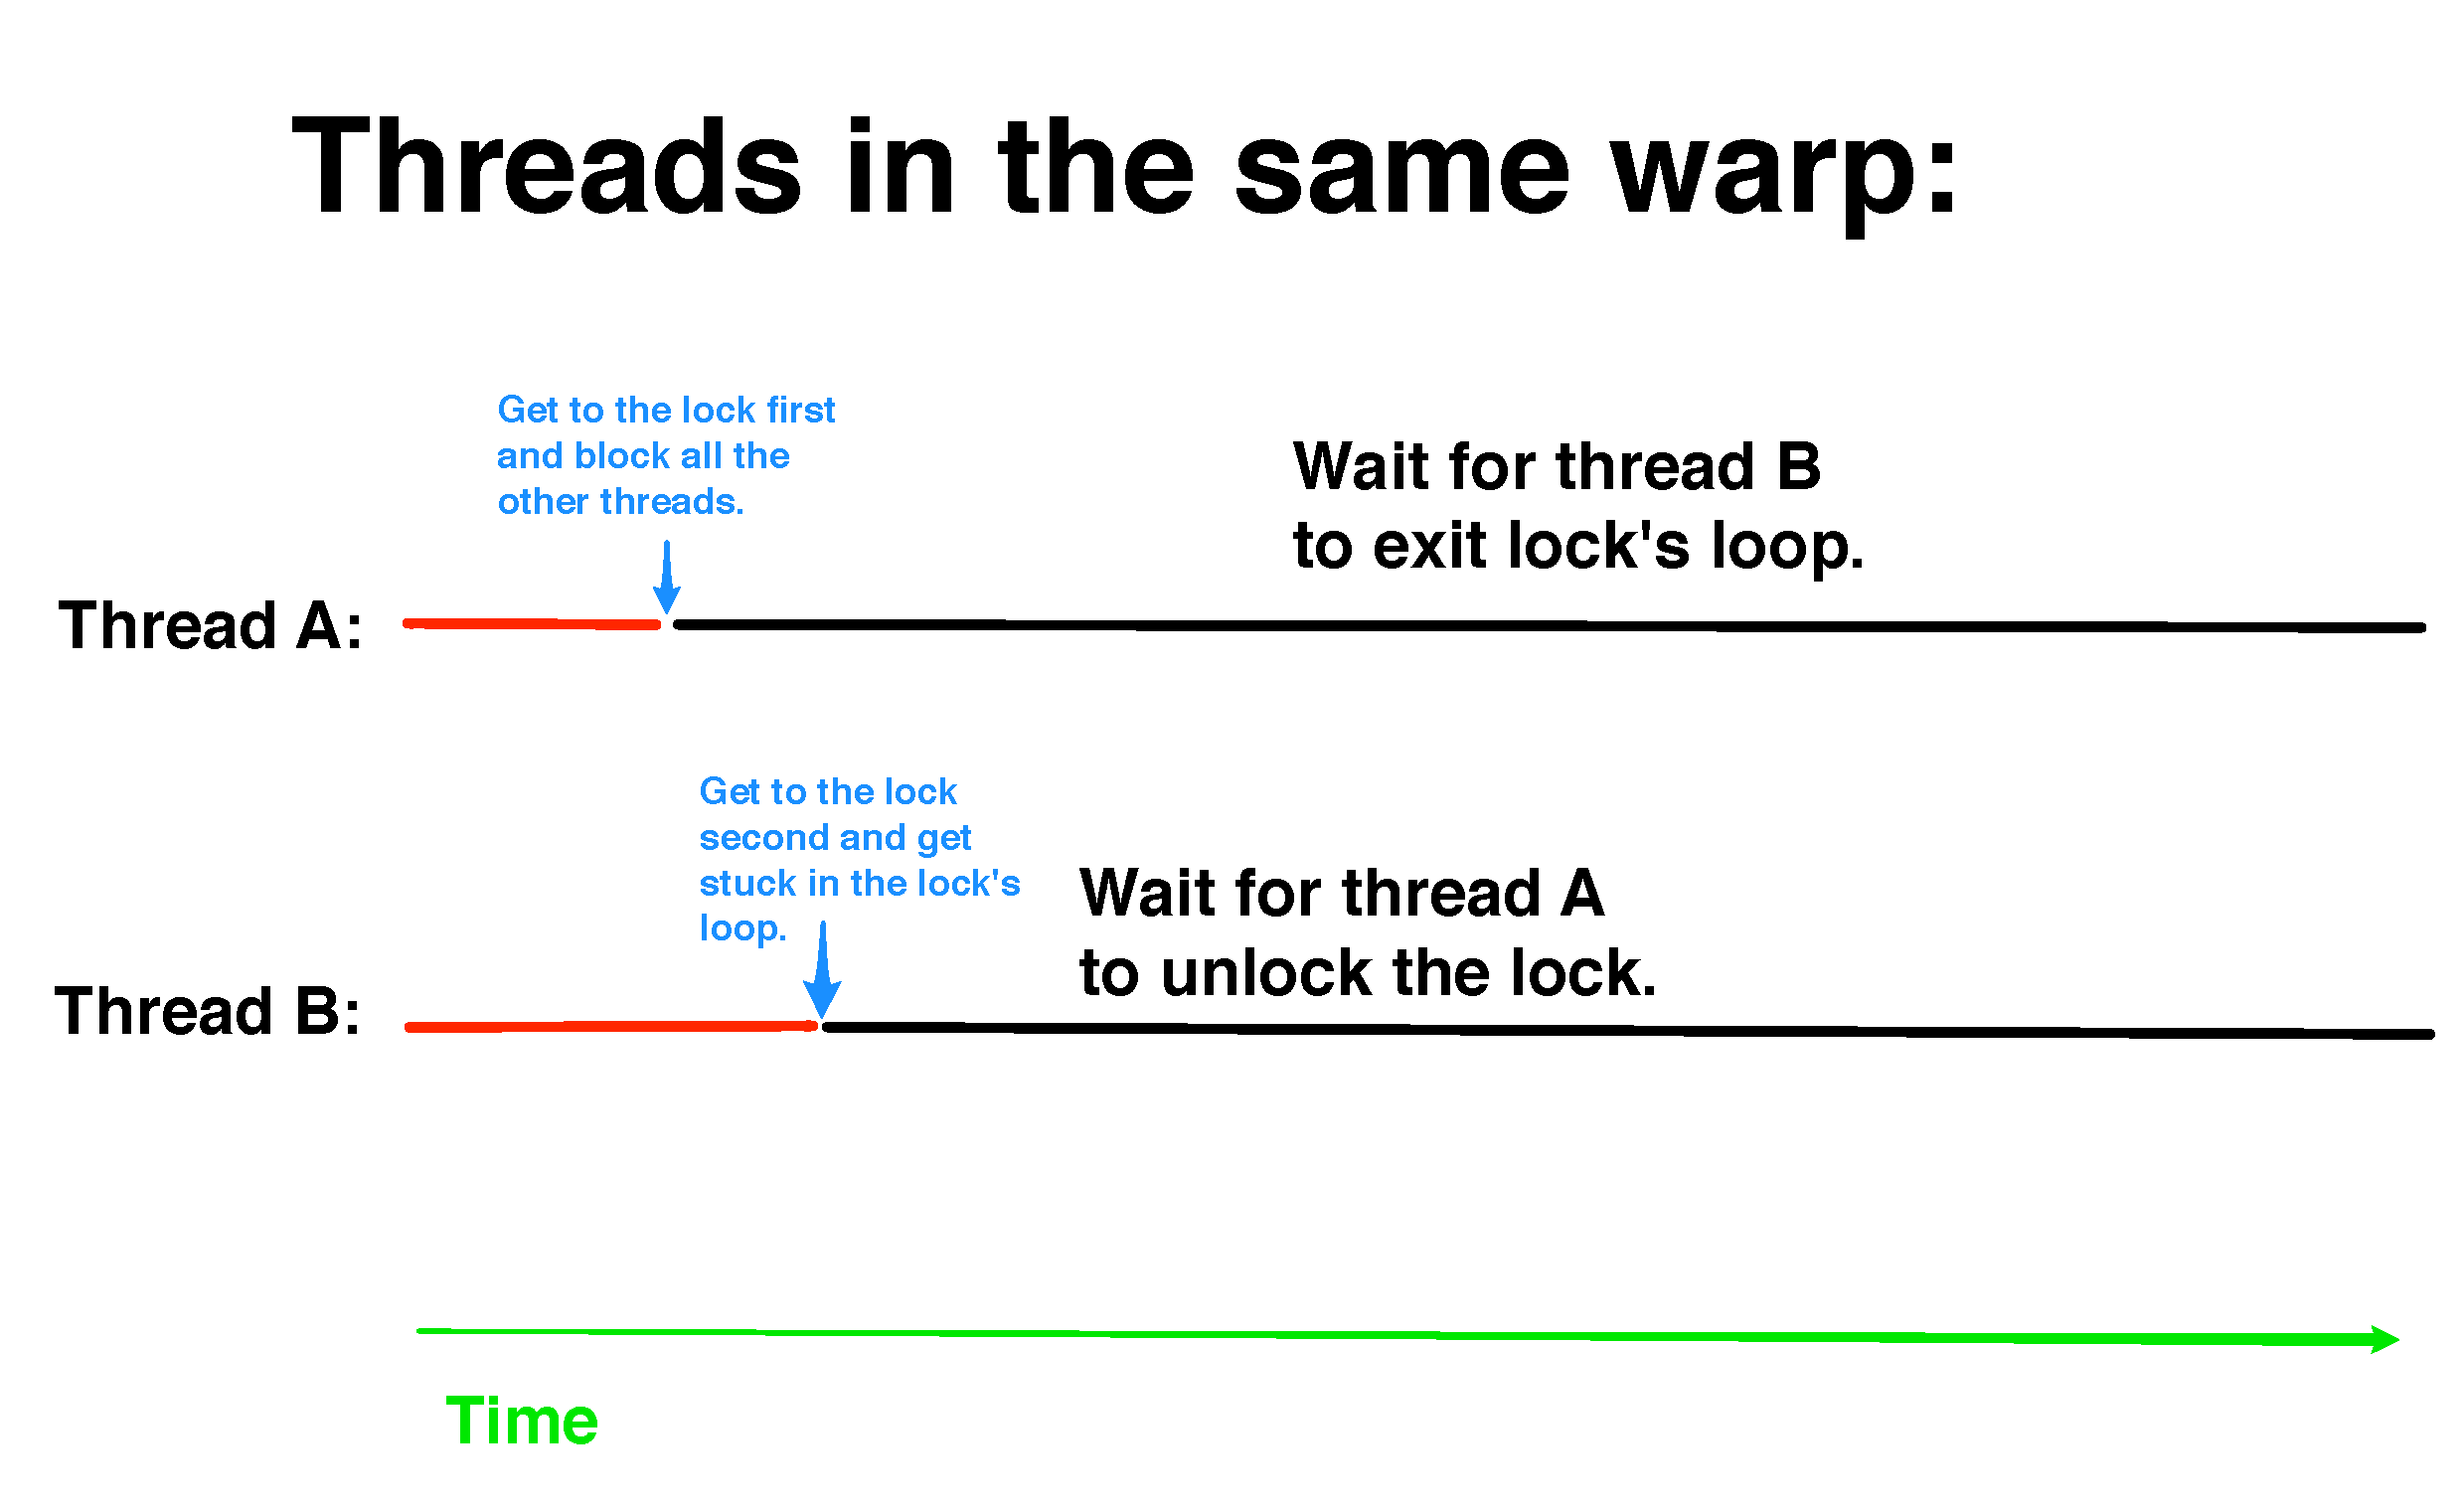
\includegraphics[scale=.2]{../../fig/lockwarp2}
\end{center}
\end{frame}

\begin{frame}
\frametitle{Outline}
\tableofcontents
\end{frame}

\begin{frame}
\frametitle{Resources} \small

\begin{itemize}
\item Texts:
\begin{enumerate}
 \item J. Sanders and E. Kandrot. {CUDA by Example.} Addison-Wesley, 2010.
\pause \item D. Kirk, W.H. Wen-mei, and W. Hwu. \emph{Programming massively parallel processors: a hands-on approach.} Morgan Kaufmann, 2010.
\end{enumerate}
\pause \item Code from today:
\begin{itemize}
\item \href{http://will-landau.com/gpu/Code/CUDA_C/race_condition/race_condition.cu}{race\_condition.cu}
\item \href{http://will-landau.com/gpu/Code/CUDA_C/race_condition_fixed/race_condition_fixed.cu}{race\_condition\_fixed.cu}
\item \href{http://will-landau.com/gpu/Code/CUDA_C/blockCounter/blockCounter.cu}{blockCounter.cu}
\end{itemize}
\pause \item Dot product with atomic operations:
\begin{itemize}
\item \href{http://will-landau.com/gpu/Code/CUDA_C/dot_product_atomic_builtin/dot_product_atomic_builtin.cu}{dot\_product\_atomic\_builtin.cu}
\item \href{http://will-landau.com/gpu/Code/CUDA_C/dot_product_atomic_lock/dot_product_atomic_lock.cu}{dot\_product\_atomic\_lock.cu}
\end{itemize}
\end{itemize}
\end{frame}


\begin{frame}
\frametitle{That's all for today.}
\begin{itemize}
\item Series materials are available at \url{http://will-landau.com/gpu}.
\end{itemize}
\end{frame}


\end{document}